\documentclass[11pt,a4paper,oneside]{article}
\usepackage{amsfonts}
\usepackage{systeme}
\usepackage{graphicx}
\usepackage[left=2cm,top=3cm]{geometry}

\begin{document}
\section*{\huge{Výstupní zpráva}}
Jméno: Josef Kuchař \\
Login: xkucha28
\section*{Architektura navrženého obvodu (na úrovni RTL)}
\subsection*{Schéma obvodu}
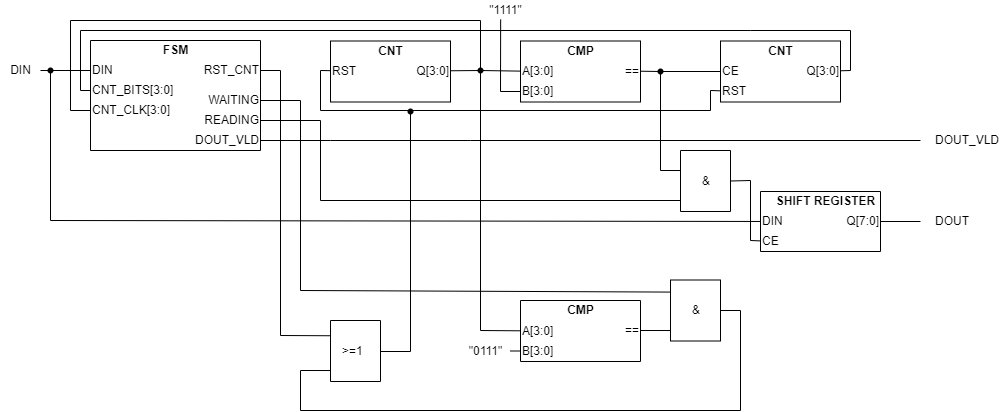
\includegraphics[width=\textwidth,height=\textheight,keepaspectratio]{schema}
\subsection*{Popis funkce}
Obvod slouží ke čtení z UART linky. Navrhnutý obvod používá FSM pro řízení chodu celého obvodu, schéma je zobrazeno níže.
Dále jsou zde dva čítače, jeden počítá hodinové cykly a druhý počítá počet přečtených bitů.
Pro výstup je použit shift register, který čte vždy po 16 cyklech, toto je zaručeno vhodně zvoleným comparatorem.
Zbytek obvodu resetuje počítadlo cyklů po průchodu 8 cykly, abychom mohli začít číst po 16 cyklech.
Konkrétnější popis je uveden níže v popisu funkce automatu.
\newpage
\section*{Návrh automatu (Finite State Machine)}
\subsection*{Schéma automatu}
Legenda
\begin{itemize}
  \item Stavy automatu: WAIT, START, RECIEVE, STOP, VALID
  \item Vstupní signály: DIN, CNT\_CLK, CNT\_BITS
  \item Moorovy výstupy: RST\_CNT, WAITING, READING, DOUT\_VLD
\end{itemize}
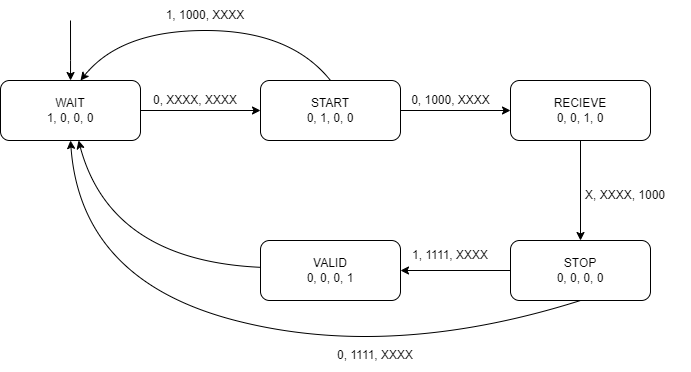
\includegraphics[width=\textwidth,height=\textheight,keepaspectratio]{fsm}
\subsection*{Popis funkce}
Automat začíná ve stavu \textbf{WAIT}. Při změně \textbf{DIN = 0} automat přejde do stavu \textbf{START}.
Ve stavu \textbf{START} se začínají počítat hodinové cykly (\textbf{CNT\_CLK}).
Jakmile \textbf{CNT\_CLK = 8} automat přejde do stavu podle \textbf{DIN}
(1 $\rightarrow$ \textbf{WAIT} - startbit je neplatný, 0 $\rightarrow$ \textbf{RECIEVE}).
Ve stavu \textbf{RECIEVE} je dokud \textbf{CNT\_BITS $<$ 8}, poté automat přejde do stavu \textbf{STOP}.
Ve stavu \textbf{STOP} čeká dalších 16 cyklů a přejde do stavu podle \textbf{DIN} (0 $\rightarrow$ \textbf{WAIT} - stopbit je neplatný, 1 $\rightarrow$ \textbf{VALID}).
Ve stavu \textbf{VALID} se zapíše na výstup, že je hodnota v shift registru validní a přejde zpět do stavu \textbf{WAIT}.
% \newpage
% \section*{Snímek obrazovky ze simulací}
\end{document}
